\begin{figure*}[t]
    \centering

    \begin{subfigure}{0.244\textwidth}
        \centering
        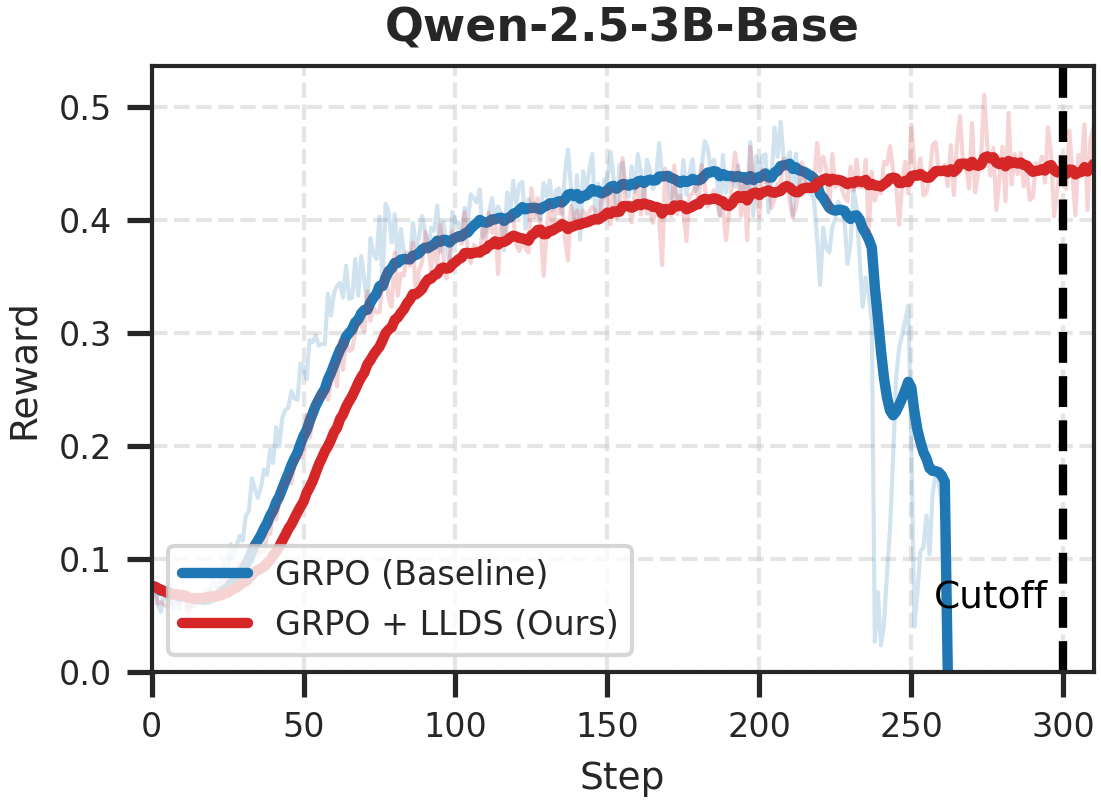
\includegraphics[width=\linewidth]{images/training_curves/comparison_3b_base.png}
        \label{fig:3b_base}
    \end{subfigure}
    \hfill
    \begin{subfigure}{0.244\textwidth}
        \centering
        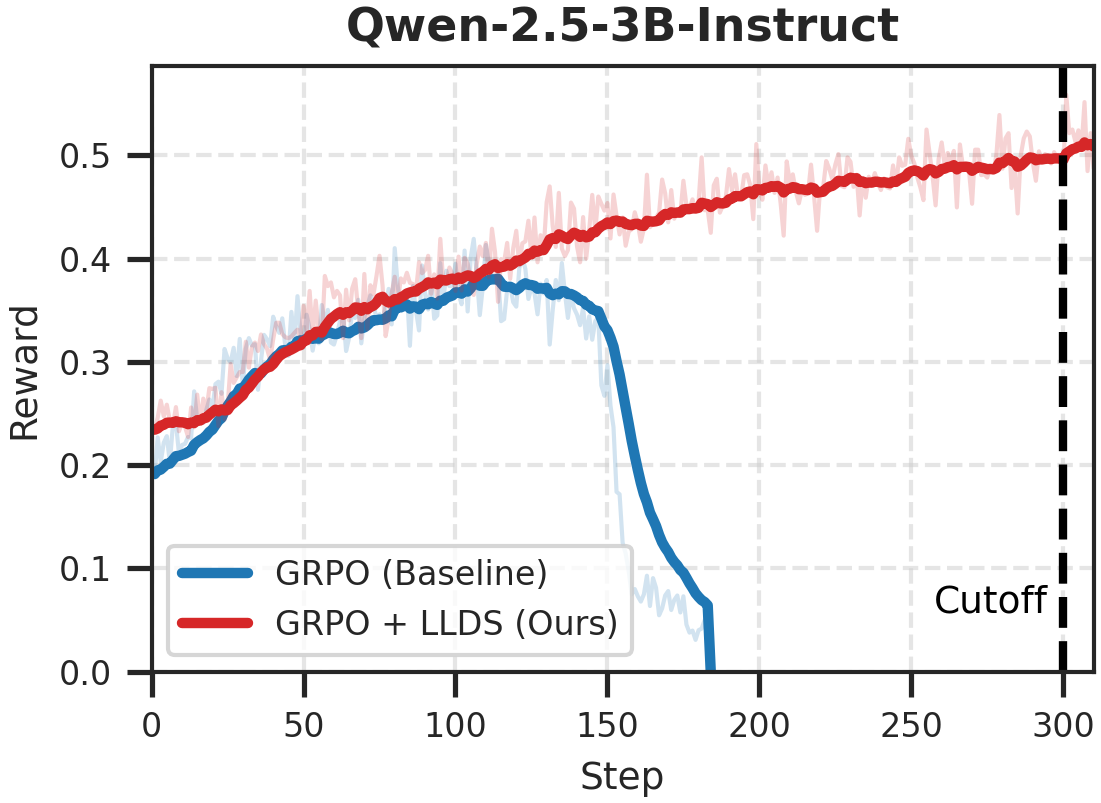
\includegraphics[width=\linewidth]{images/training_curves/comparison_3b_instruct.png}
        \label{fig:3b_instruct}
    \end{subfigure}
    \hfill
    \begin{subfigure}{0.244\textwidth}
        \centering
        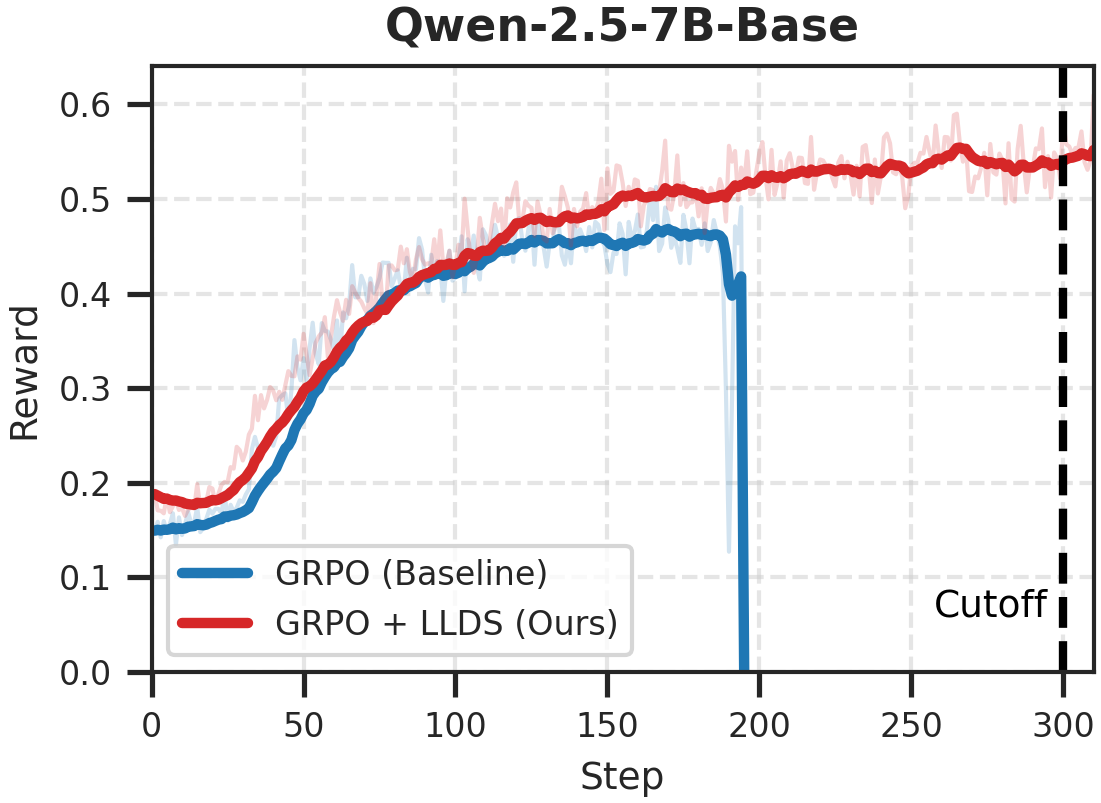
\includegraphics[width=\linewidth]{images/training_curves/comparison_7b_base.png}
        \label{fig:7b_base}
    \end{subfigure}
    \hfill
    \begin{subfigure}{0.244\textwidth}
        \centering
        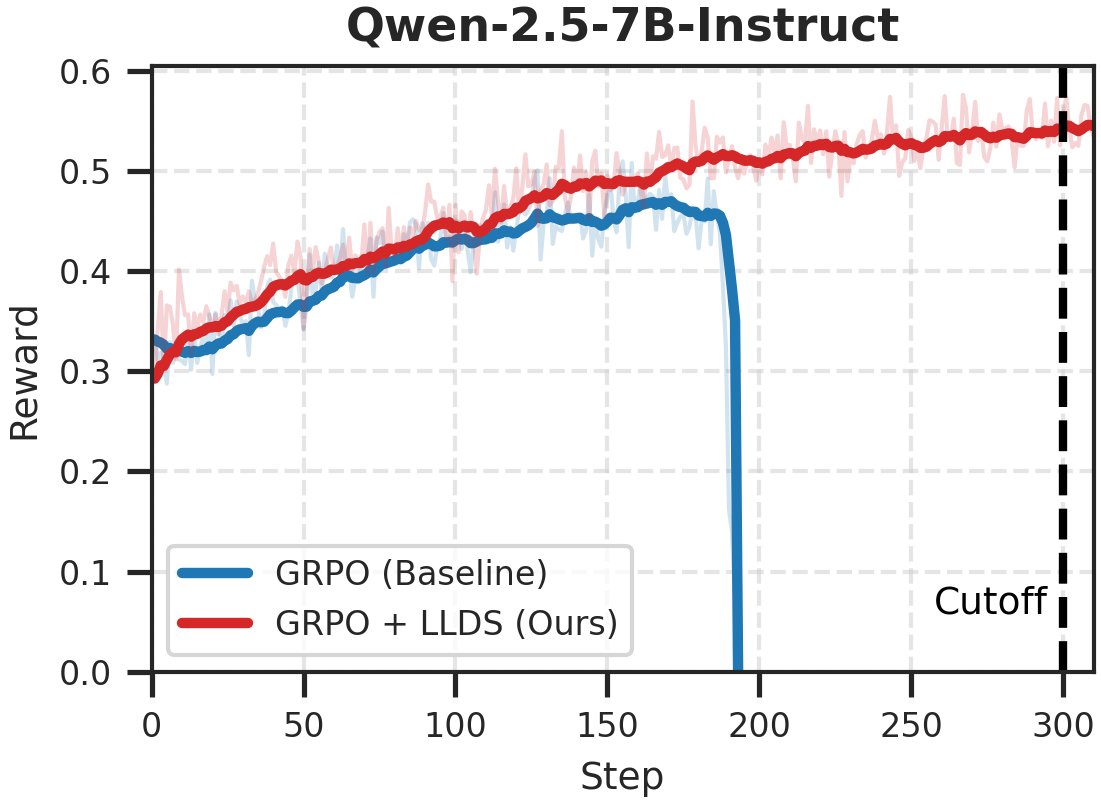
\includegraphics[width=\linewidth]{images/training_curves/comparison_7b_instruct.png}
        \label{fig:7b_instruct}
    \end{subfigure}

    \vspace{-1.5em}
    \caption{Comparisons of training reward curves between baseline GRPO (\textcolor{blue}{blue}) and GRPO + LLDS (\textcolor{red}{red}). 
    From left to right: Qwen-2.5-3B-Base, Qwen-2.5-3B-Instruct, Qwen-2.5-7B-Base, and Qwen-2.5-7B-Instruct. 
    The baseline consistently collapses (reward drops to zero), while LLDS stabilizes training and sustains high rewards.}
    \label{fig:comparison_curves}
    \vspace{-4mm}
\end{figure*}


\subsection{Experimental Results}\label{sec:reuslt}
We evaluate our proposed \ours{} on seven open-domain and multi-hop QA benchmarks using two model families: Qwen2.5-3B (Base/Instruct) and Qwen2.5-7B (Base/Instruct). Tables~\ref{tab:qa_results_3b} and~\ref{tab:qa_results} summarize the EM performance across all settings. Since vanilla GRPO training often collapses, we use the results from Search-R1~\cite{jin2025search}, corresponding to the best checkpoint before collapse, as the GRPO baseline. This choice favors GRPO and avoids underestimating its performance. More results see~\cref{sec:add_result}.
\\
\textbf{Results on Qwen2.5-3B.} As shown in \cref{tab:qa_results_3b}, \ours{} improves the vanilla GRPO score from 0.312 to 0.360, corresponding to a 15.4\% relative gain. Notably, because the 3B base model tends to invoke search only once, we apply \ours{}-MA, which achieves the best performance with an average score of 0.440, representing a substantial +45.2\% improvement over GRPO. A similar trend is observed for Qwen2.5-3B-Instruct, where LLDS attains 0.441 under the NQ+Hotpot setting (+31.3\%).
\\
\textbf{Results on Qwen2.5-7B.}
As shown in \cref{tab:qa_results}, \ours{} delivers substantial gains over vanilla GRPO for both base and instruct variants. For Qwen2.5-7B-Base, it improves the average score from 0.350 to 0.480, a 37.1\% relative increase, while for Qwen2.5-7B-Instruct, performance rises from 0.396 to 0.483, corresponding to a 22.0\% gain. Notably, \ours{} attains the best results on all Multi-Hop QA benchmarks with MH-Avg accuracy being 0.426.
\\
\textbf{Comparison with Dense Rewards.}
As shown in \cref{tab:qa_results_3b,tab:qa_results}, stabilizing outcome-reward GRPO training with \ours{} consistently outperforms methods that rely on dense reward supervision. These dense-reward approaches typically require turn-level ground-truth signals, external LLM judges, or more expensive tree-based rollouts. In contrast, \ours{} achieves superior performance using only outcome rewards. Notably, \ours{} outperforms the strongest dense-reward baseline, Tree-GRPO, by 4\% and 10\% on the 3B and 7B models, respectively, and exceeds other dense-reward methods by over 30\%, demonstrating both improved effectiveness and substantially lower supervision.
\\ 
\textbf{Results on GSPO.} We further show that \ours{} integrates seamlessly with other group-relative reinforcement learning objectives. In particular, we apply \ours{} to Group Sequence Policy Optimization (GSPO)~\citep{zheng2025group}, which optimizes sequence-level importance ratios. As shown in Table~\ref{tab:qa_results_3b}, vanilla GSPO also suffers from limited performance due to training collapse, whereas incorporating \ours{} consistently improves results across both General QA and Multi-Hop QA benchmarks. Notably, GSPO+\ours{} achieves the highest overall average score (0.451) on Qwen2.5-3B-Instruct, outperforming GSPO by 36.3\%. These results confirm the generality of \ours{} across group-relative optimization formulations.
\subsection{Ablation Study and Analysis}% \textbf{Impact of response-level gating.}
% Applying response-level gating reduces the strength of the regularization applied during training, leading to measurable improvements on multi-hop QA tasks. As shown in \cref{tab:qa_results_3b}, although the average performance increases modestly by 0.2\%, the method yields a notable 1.6\% gain on the Bamboogle dataset, highlighting its effectiveness in enhancing multi-hop reasoning.
% \\
\vspace{-1mm}
\textbf{Impact of Regularization Strength.}
We ablate $\lambda \in \{0, 0.01, 0.1, 0.2\}$ and plot the corresponding training reward dynamics in \cref{fig:strength_nqhot}. As shown, Vanilla GRPO ($\lambda = 0$) collapses around step 200. A small regularization value ($\lambda = 0.01$, orange curve) delays but does not prevent collapse, which occurs around step 220. In contrast, a stronger regularization ($\lambda = 0.2$) stabilizes training entirely, allowing the model to continue smoothly without collapse. We truncate the plot at step 500 for clarity, although training can proceed well beyond this point.
\begin{figure}[t]
    \centering
    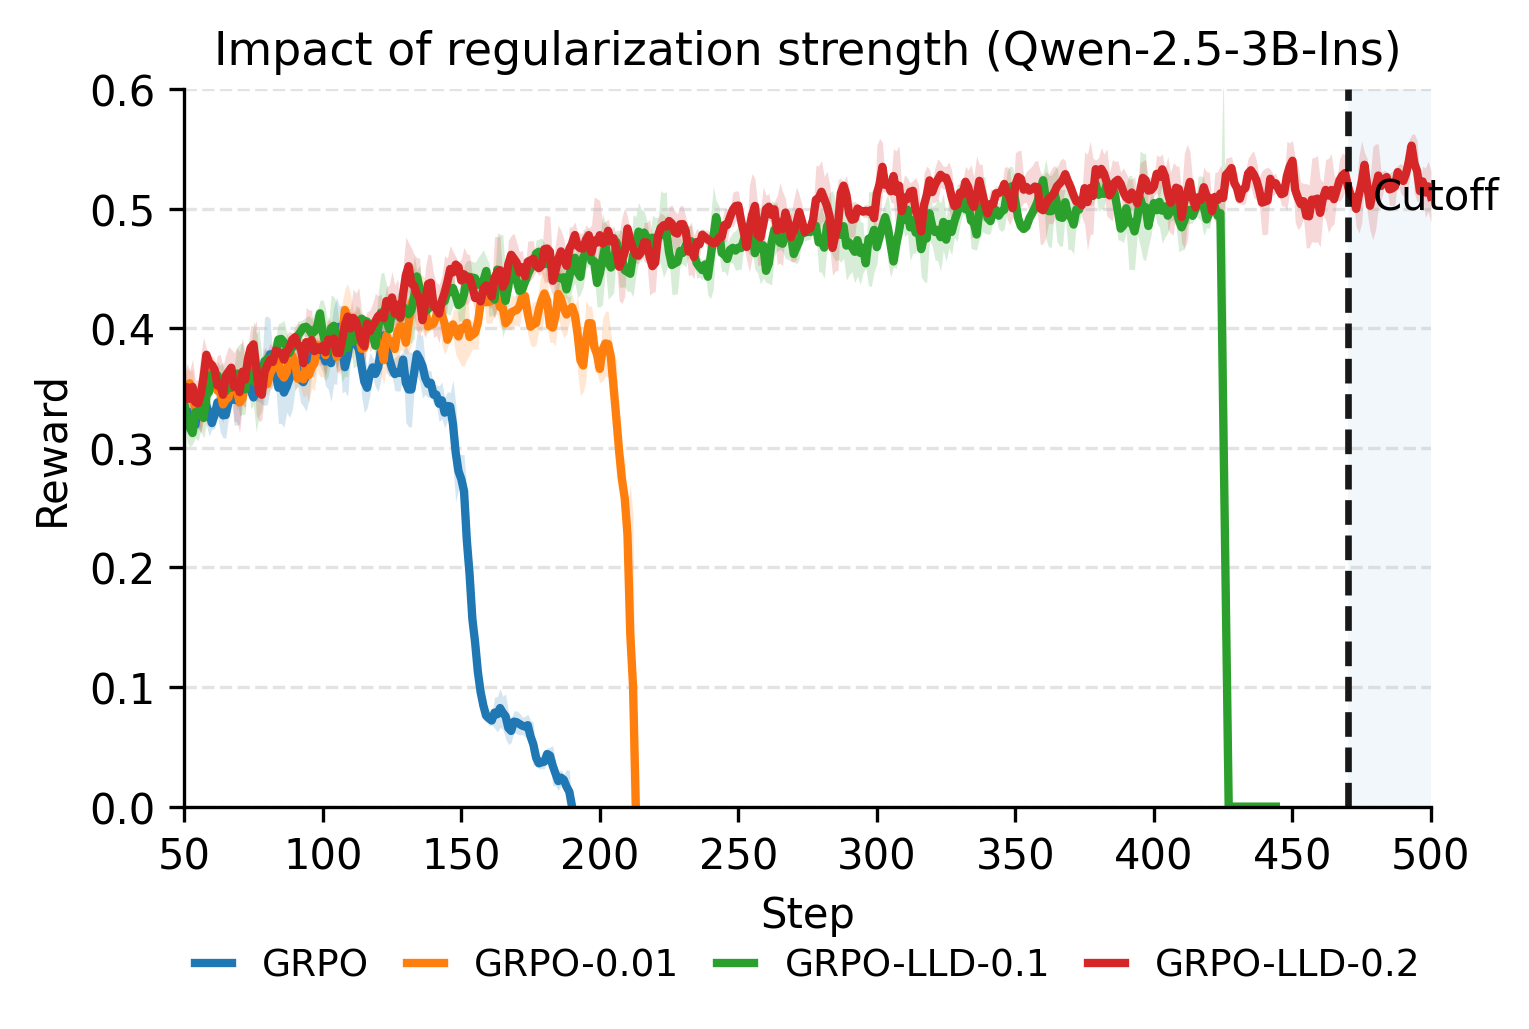
\includegraphics[width=\linewidth]{images/3bins-reg-strength.png}
    \vspace{-3mm}
        \caption{Impact of regularization strength in training Qwen2.5-3B-Instruct on NQ and HotpotQA.}
    \label{fig:strength_nqhot}
    \vspace{-6mm}
\end{figure}
\\
\textbf{Impact of masking answer (MA).}
We apply MA only to model variants where vanilla GRPO degenerate into issuing only a single search call. MA reduces LLDS regularization on the final answer tokens, encouraging the model to perform additional search steps or intermediate reasoning. As shown in \cref{tab:qa_results_3b}, LLDS-MA increases the Qwen2.5-3B-Base average score in the NQ+Hotpot setting from 0.360 (LLDS) to 0.430. These gains demonstrate that MA effectively encourages deeper, multi-step reasoning in scenarios where the underlying GRPO policy underutilizes search actions. More detailed analysis see~\cref{sec:mask_answer}.
\\
\textbf{Effect of LLDS on Training Stability across Models}
\label{sec:effect_llds}
To assess the universality of GRPO collapse and the robustness of our method, we evaluate across model scales (3B and 7B) and alignment stages (Base and Instruct). As shown in \Cref{fig:comparison_curves}, vanilla GRPO consistently collapses within the first 300 steps regardless of model size or variant. In contrast, integrating \ours{} (red line) reliably stabilizes training and maintains steady reward growth across all four settings, successfully avoiding the collapse issue. These results demonstrate that \ours{} serves as a general and effective regularizer for stabilizing GRPO training.

